\documentclass[11pt,oneside]{book}

\usepackage[margin=1in]{geometry}
\usepackage[T1]{fontenc}
\usepackage[utf8]{inputenc}
\usepackage{lmodern}
\usepackage{microtype}
\usepackage{amsmath,amssymb,amsthm,mathtools,bm}
\usepackage{booktabs,array,tabularx,longtable}
\usepackage{enumitem}
\usepackage{xcolor}
\usepackage[most]{tcolorbox}
\usepackage{tikz}
\usepackage{pgfplots}
\usepackage{pgfplotstable}
\usepackage{tikz-3dplot}
\usepackage{float}
\usepackage{caption}
\usepackage{fancyhdr}
\usepackage{hyperref}
\usepackage{xurl}

\pgfplotsset{compat=1.18}
\usepgfplotslibrary{fillbetween}
\usetikzlibrary{arrows.meta,calc,positioning,intersections,patterns,decorations.pathreplacing,backgrounds,fit,matrix,shapes.geometric}

\definecolor{chapterblue}{HTML}{1F5AA6}
\definecolor{chapterteal}{HTML}{168A8F}
\definecolor{chapterorange}{HTML}{D9822B}
\definecolor{chaptergreen}{HTML}{2D8A4E}
\definecolor{chapterpurple}{HTML}{6B4EAA}
\definecolor{chapterred}{HTML}{B23B3B}
\definecolor{softblue}{HTML}{EAF3FF}
\definecolor{softgreen}{HTML}{EAF8EF}
\definecolor{softorange}{HTML}{FFF4E6}
\definecolor{softpurple}{HTML}{F3EEFF}
\definecolor{softred}{HTML}{FFF0F0}
\definecolor{softgray}{HTML}{F6F7F9}
\definecolor{darkgray}{HTML}{30343B}

\hypersetup{
  colorlinks=true,
  linkcolor=chapterblue,
  urlcolor=chapterteal,
  citecolor=chapterpurple,
  pdftitle={Chapter 24. Multivariable Calculus for Probability and Statistics},
  pdfauthor={He Wang}
}

\setlength{\parindent}{0pt}
\setlength{\parskip}{0.62em}
\setlength{\headheight}{14pt}
\setlist[itemize]{topsep=2pt,itemsep=2pt,leftmargin=1.5em}
\setlist[enumerate]{topsep=2pt,itemsep=2pt,leftmargin=1.7em}

\pagestyle{fancy}
\fancyhf{}
\fancyhead[L]{\small\textsc{Chapter 24. Probability and Statistics}}
\fancyhead[R]{\small\thepage}
\renewcommand{\headrulewidth}{0.4pt}

\tikzset{
  vector/.style={-Latex,very thick,chapterblue},
  vectorred/.style={-Latex,very thick,chapterred},
  vectorteal/.style={-Latex,very thick,chapterteal},
  vectororange/.style={-Latex,very thick,chapterorange},
  guide/.style={thin,dashed,darkgray!55},
  point/.style={circle,fill=chapterblue,inner sep=1.4pt},
  redpoint/.style={circle,fill=chapterred,inner sep=1.4pt},
  boxnode/.style={draw=chapterblue!70!black,fill=softblue,rounded corners=2mm,align=center,inner sep=5pt},
  greennode/.style={draw=chaptergreen!70!black,fill=softgreen,rounded corners=2mm,align=center,inner sep=5pt},
  orangenode/.style={draw=chapterorange!75!black,fill=softorange,rounded corners=2mm,align=center,inner sep=5pt},
  purplenode/.style={draw=chapterpurple!75!black,fill=softpurple,rounded corners=2mm,align=center,inner sep=5pt},
  rednode/.style={draw=chapterred!75!black,fill=softred,rounded corners=2mm,align=center,inner sep=5pt}
}

\newtcolorbox{mainideabox}[1][]{
  enhanced,breakable,
  colback=softblue,
  colframe=chapterblue,
  title=#1,
  fonttitle=\bfseries,
  boxrule=0.8pt,
  arc=2mm,
  left=2mm,right=2mm,top=1mm,bottom=1mm
}

\newtcolorbox{definitionbox}[1][]{
  enhanced,breakable,
  colback=softgreen,
  colframe=chaptergreen,
  title=#1,
  fonttitle=\bfseries,
  boxrule=0.8pt,
  arc=2mm,
  left=2mm,right=2mm,top=1mm,bottom=1mm
}

\newtcolorbox{examplebox}[1]{
  enhanced,breakable,
  colback=white,
  colframe=chapterblue,
  colbacktitle=chapterblue,
  coltitle=white,
  title={#1},
  fonttitle=\bfseries,
  boxrule=0.8pt,
  arc=2mm,
  left=2mm,right=2mm,top=1mm,bottom=1mm
}

\newtcolorbox{notebox}[1][]{
  enhanced,breakable,
  colback=softpurple,
  colframe=chapterpurple,
  title=#1,
  fonttitle=\bfseries,
  boxrule=0.8pt,
  arc=2mm,
  left=2mm,right=2mm,top=1mm,bottom=1mm
}

\newtcolorbox{tipbox}[1][]{
  enhanced,breakable,
  colback=softorange,
  colframe=chapterorange,
  title=#1,
  fonttitle=\bfseries,
  boxrule=0.8pt,
  arc=2mm,
  left=2mm,right=2mm,top=1mm,bottom=1mm
}

\newtcolorbox{warningbox}[1][]{
  enhanced,breakable,
  colback=softred,
  colframe=chapterred,
  title=#1,
  fonttitle=\bfseries,
  boxrule=0.8pt,
  arc=2mm,
  left=2mm,right=2mm,top=1mm,bottom=1mm
}

\newcommand{\R}{\mathbb R}
\newcommand{\E}{\mathbb E}
\newcommand{\Prob}{\mathbb P}
\newcommand{\Var}{\operatorname{Var}}
\newcommand{\Cov}{\operatorname{Cov}}
\newcommand{\diag}{\operatorname{diag}}
\newcommand{\dd}{\,d}
\newcommand{\grad}{\nabla}
\newcommand{\norm}[1]{\left\lVert #1\right\rVert}
\newcommand{\abs}[1]{\left\lvert #1\right\rvert}

\begin{document}
\setcounter{chapter}{23}
\chapter{Multivariable Calculus for Probability and Statistics}
\textit{Densities, expectations, transformations, likelihood, and local approximation}

Probability and statistics give one of the most important modern uses of multivariable calculus. A probability model is often a function on a space of possible outcomes. A statistical model is often a function on a space of unknown parameters. In both cases, we need the language of multivariable calculus: domains, level curves, multiple integrals, gradients, Hessians, Jacobians, and change of variables.

This chapter is a bridge from the core calculus of several variables to later courses in probability, mathematical statistics, data science, and machine learning. The central idea is simple.

\begin{mainideabox}[Central idea]
A density is a function whose integral gives probability. A likelihood is a function whose maximum gives an estimate.
\end{mainideabox}

The first sentence uses multiple integrals. The second uses gradients and optimization.

\begin{figure}[H]
\centering
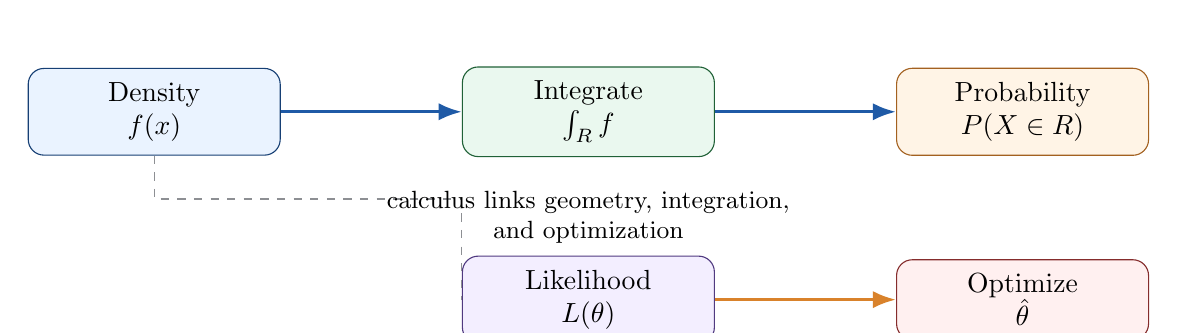
\begin{tikzpicture}[node distance=1.8cm]
  \node[boxnode,minimum width=3.2cm] (density) {Density\\$f(x)$};
  \node[greennode,right=2.3cm of density,minimum width=3.2cm] (integral) {Integrate\\$\int_R f$};
  \node[orangenode,right=2.3cm of integral,minimum width=3.2cm] (prob) {Probability\\$P(X\in R)$};
  \node[purplenode,below=1.25cm of integral,minimum width=3.2cm] (like) {Likelihood\\$L(\theta)$};
  \node[rednode,right=2.3cm of like,minimum width=3.2cm] (opt) {Optimize\\$\hat\theta$};
  \draw[vector] (density) -- (integral);
  \draw[vector] (integral) -- (prob);
  \draw[vectororange] (like) -- (opt);
  \draw[guide] (density.south) -- ++(0,-0.55) -| (like.west);
  \node[align=center,font=\small] at ($(integral)!0.5!(like)+(0,-0.15)$) {calculus links geometry, integration,\\and optimization};
\end{tikzpicture}
\caption{Two central roles of multivariable calculus in statistics: integration over outcome space and optimization over parameter space.}
\end{figure}

\section*{Learning goals}
After studying this chapter, you should be able to:
\begin{enumerate}
  \item interpret a joint density $f_{X,Y}(x,y)$ geometrically and probabilistically;
  \item compute probabilities and expectations using double and triple integrals;
  \item find marginal and conditional densities from a joint density;
  \item use change of variables and Jacobians to transform random variables;
  \item interpret covariance matrices through ellipses and quadratic forms;
  \item use gradients and Hessians to understand likelihood functions;
  \item connect Taylor approximation to standard errors and uncertainty quantification;
  \item use numerical integration and simulation to check analytic calculations.
\end{enumerate}

Throughout the chapter, keep two pictures in mind. A joint density is like a surface whose total volume is $1$. A log-likelihood is like a landscape whose highest point gives the best-fitting parameter.

\section{Random variables as functions and data as points}

A random variable is a function from a sample space to numbers. A random vector is a function from a sample space to a vector space.

For example, if we observe height and weight from a randomly selected person, then the outcome can be written as a vector
\[
X=(X_1,X_2)=(\text{height},\text{weight})\in\R^2.
\]
If we observe $n$ measurements, the dataset can be written as a point in $\R^n$:
\[
x=(x_1,x_2,\ldots,x_n).
\]
If we fit a model with parameters $\theta_1,\ldots,\theta_p$, the parameter vector is a point in parameter space:
\[
\theta=(\theta_1,\ldots,\theta_p)\in\R^p.
\]
This is why multivariable calculus appears everywhere in statistics. We integrate over outcome spaces, differentiate over parameter spaces, and use linear and quadratic approximations to measure uncertainty.

\begin{notebox}[Three spaces in statistics]
A statistical problem often involves three different spaces:
\begin{itemize}
  \item \textbf{Sample space:} where random outcomes live.
  \item \textbf{Data space:} where observed datasets live.
  \item \textbf{Parameter space:} where unknown model parameters live.
\end{itemize}
Multivariable calculus helps us move among all three.
\end{notebox}

\begin{figure}[H]
\centering
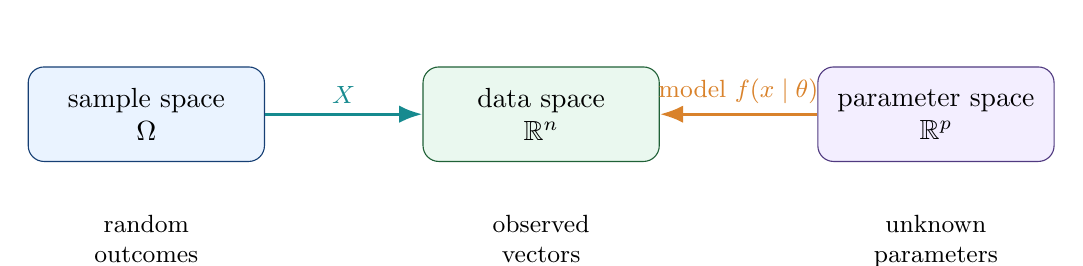
\begin{tikzpicture}[node distance=1.4cm]
  \node[boxnode,minimum width=3.0cm,minimum height=1.2cm] (sample) {sample space\\$\Omega$};
  \node[greennode,right=2.0cm of sample,minimum width=3.0cm,minimum height=1.2cm] (data) {data space\\$\R^n$};
  \node[purplenode,right=2.0cm of data,minimum width=3.0cm,minimum height=1.2cm] (param) {parameter space\\$\R^p$};
  \draw[vectorteal] (sample) -- node[above,font=\small] {$X$} (data);
  \draw[vectororange] (param) -- node[above,font=\small] {model $f(x\mid\theta)$} (data);
  \node[below=0.55cm of sample,align=center,font=\small] {random\\outcomes};
  \node[below=0.55cm of data,align=center,font=\small] {observed\\vectors};
  \node[below=0.55cm of param,align=center,font=\small] {unknown\\parameters};
\end{tikzpicture}
\caption{Statistics moves among sample space, data space, and parameter space. Multivariable calculus supplies the geometry and computation.}
\end{figure}

\section{Joint densities and probability as volume}

A continuous random vector $(X,Y)$ has a joint density $f_{X,Y}(x,y)$ if probabilities are computed by double integrals:
\[
\Prob((X,Y)\in R)=\iint_R f_{X,Y}(x,y)\dd A.
\]
For $f_{X,Y}$ to be a valid density, it must satisfy
\[
f_{X,Y}(x,y)\ge 0,
\qquad
\iint_{\R^2} f_{X,Y}(x,y)\dd A=1.
\]
The probability of a region is the volume under the density surface above that region.

\begin{examplebox}{Example 24.1: A simple density on a square}
Let
\[
f(x,y)=x+y
\]
on the unit square $0\le x\le 1$, $0\le y\le 1$, and let $f(x,y)=0$ outside the square. This is a probability density because
\[
\int_0^1\int_0^1(x+y)\dd y\dd x
=\int_0^1\left(x+\frac12\right)\dd x=1.
\]
Now compute $\Prob(X+Y\le 1)$. The region is the triangle $0\le x\le 1$, $0\le y\le 1-x$. Thus
\[
\Prob(X+Y\le 1)=\int_0^1\int_0^{1-x}(x+y)\dd y\dd x.
\]
The inner integral is
\[
\int_0^{1-x}(x+y)\dd y=x(1-x)+\frac{(1-x)^2}{2}.
\]
Therefore,
\[
\Prob(X+Y\le 1)=\int_0^1\left[x(1-x)+\frac{(1-x)^2}{2}\right]\dd x=\frac12.
\]
\end{examplebox}

\begin{figure}[H]
\centering
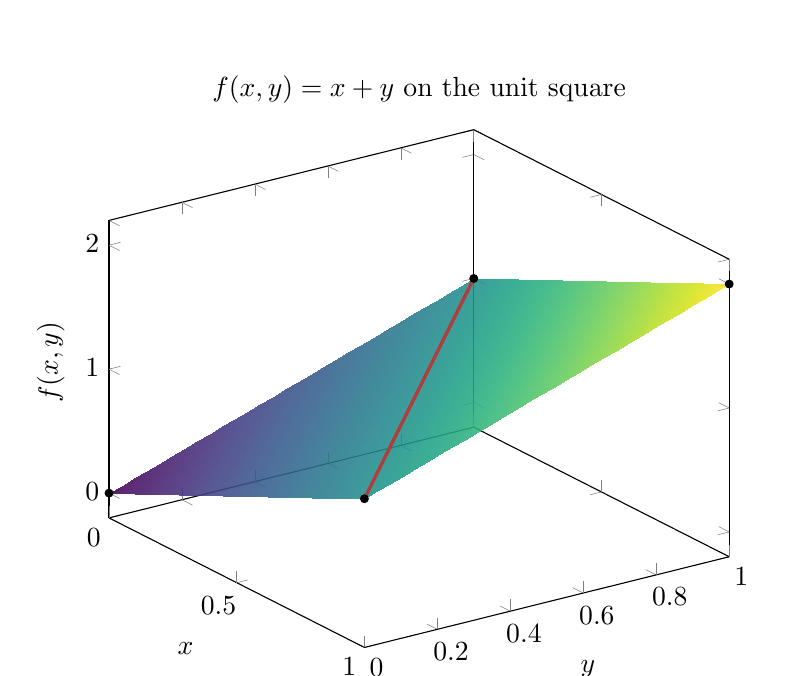
\begin{tikzpicture}
\begin{axis}[
  width=0.78\textwidth,
  view={55}{28},
  xlabel={$x$},ylabel={$y$},zlabel={$f(x,y)$},
  domain=0:1,y domain=0:1,
  samples=30,samples y=30,
  z buffer=sort,
  colormap/viridis,
  title={$f(x,y)=x+y$ on the unit square}
]
\addplot3[surf,shader=interp,opacity=0.88] {x+y};
\addplot3[very thick,chapterred,domain=0:1,samples=80] ({x},{1-x},{1});
\addplot3[only marks,mark=*,mark size=1.4pt] coordinates {(0,0,0) (1,0,1) (0,1,1) (1,1,2)};
\end{axis}
\end{tikzpicture}
\caption{The density $f(x,y)=x+y$ on the unit square. Probability over a region is volume under the surface over that region.}
\end{figure}

\section{Marginal densities}

A joint density describes the simultaneous behavior of two random variables. A marginal density describes one variable alone. If $(X,Y)$ has joint density $f_{X,Y}$, then the marginal density of $X$ is
\[
f_X(x)=\int_{-\infty}^{\infty} f_{X,Y}(x,y)\dd y.
\]
Similarly,
\[
f_Y(y)=\int_{-\infty}^{\infty} f_{X,Y}(x,y)\dd x.
\]
The operation is geometric: we collapse the density surface in one direction by integrating out the other variable.

\begin{examplebox}{Example 24.2: Marginals for $f(x,y)=x+y$}
On the unit square,
\[
f_X(x)=\int_0^1(x+y)\dd y=x+\frac12.
\]
Similarly,
\[
f_Y(y)=\int_0^1(x+y)\dd x=y+\frac12.
\]
Check normalization:
\[
\int_0^1 f_X(x)\dd x=\int_0^1\left(x+\frac12\right)\dd x=1.
\]
\end{examplebox}

\begin{figure}[H]
\centering
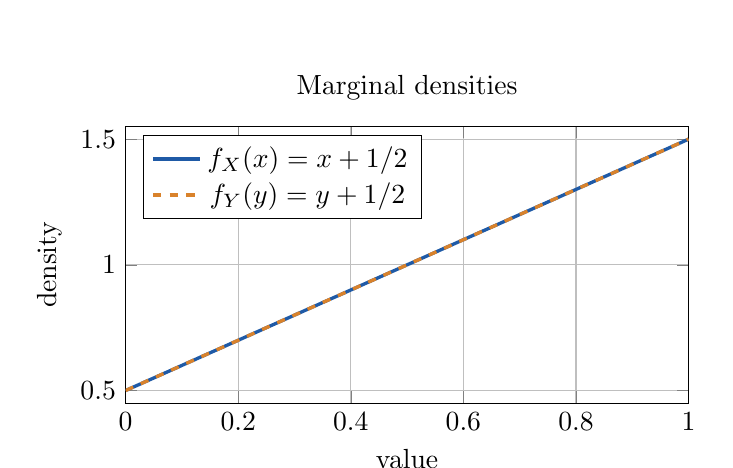
\begin{tikzpicture}
\begin{axis}[
  width=0.72\textwidth,height=0.42\textwidth,
  xmin=0,xmax=1,ymin=0.45,ymax=1.55,
  xlabel={value},ylabel={density},
  grid=both,
  legend pos=north west,
  title={Marginal densities}
]
\addplot[very thick,chapterblue,domain=0:1,samples=80] {x+0.5};
\addlegendentry{$f_X(x)=x+1/2$}
\addplot[very thick,chapterorange,dashed,domain=0:1,samples=80] {x+0.5};
\addlegendentry{$f_Y(y)=y+1/2$}
\end{axis}
\end{tikzpicture}
\caption{Marginal densities are obtained by integrating the joint density in one variable.}
\end{figure}

\begin{tipbox}[Integrating out variables]
In statistics and machine learning, the phrase \textbf{integrate out} means to remove a variable by integration. Marginalization is integration.
\end{tipbox}

\section{Conditional densities and independence}

The conditional density of $Y$ given $X=x$ is
\[
f_{Y\mid X}(y\mid x)=\frac{f_{X,Y}(x,y)}{f_X(x)},
\]
provided $f_X(x)>0$. This is the continuous analogue of conditional probability:
\[
\Prob(A\mid B)=\frac{\Prob(A\cap B)}{\Prob(B)}.
\]

\begin{examplebox}{Example 24.3: Conditional density from a joint density}
For $f(x,y)=x+y$ on the unit square,
\[
f_{Y\mid X}(y\mid x)=\frac{x+y}{x+1/2},\qquad 0\le y\le 1.
\]
For fixed $x$, this is a density in $y$:
\[
\int_0^1\frac{x+y}{x+1/2}\dd y=\frac{x+1/2}{x+1/2}=1.
\]
The conditional mean of $Y$ given $X=x$ is
\[
\E[Y\mid X=x]=\int_0^1 y\,\frac{x+y}{x+1/2}\dd y=\frac{x/2+1/3}{x+1/2}.
\]
This conditional mean depends on $x$, so knowing $X$ changes the distribution of $Y$.
\end{examplebox}

Random variables $X$ and $Y$ are independent if
\[
f_{X,Y}(x,y)=f_X(x)f_Y(y)
\]
for all relevant $(x,y)$. For $f(x,y)=x+y$, we have
\[
f_X(x)f_Y(y)=\left(x+\frac12\right)\left(y+\frac12\right),
\]
which is not equal to $x+y$. Therefore, $X$ and $Y$ are not independent.

\begin{figure}[H]
\centering
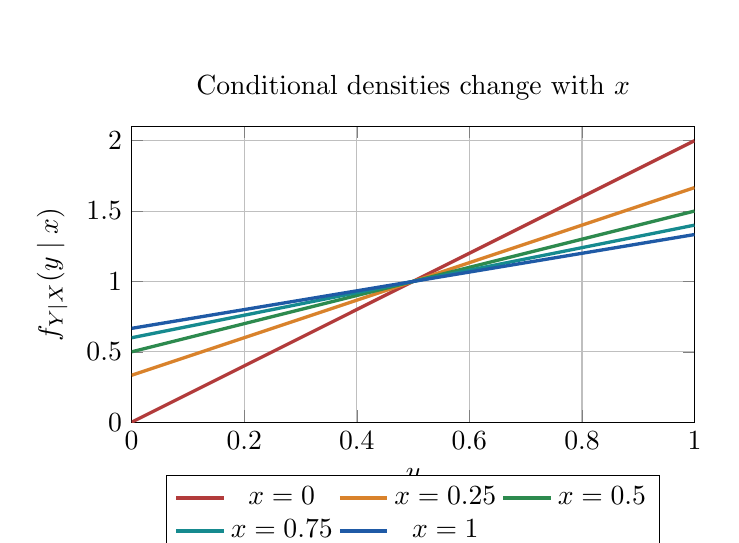
\begin{tikzpicture}
\begin{axis}[
  width=0.72\textwidth,height=0.44\textwidth,
  xmin=0,xmax=1,ymin=0,ymax=2.1,
  xlabel={$y$},ylabel={$f_{Y\mid X}(y\mid x)$},
  grid=both,
  legend columns=3,
  legend style={at={(0.5,-0.18)},anchor=north},
  title={Conditional densities change with $x$}
]
\addplot[very thick,chapterred,domain=0:1,samples=80] {(0+x)/(0+0.5)};
\addlegendentry{$x=0$}
\addplot[very thick,chapterorange,domain=0:1,samples=80] {(0.25+x)/(0.25+0.5)};
\addlegendentry{$x=0.25$}
\addplot[very thick,chaptergreen,domain=0:1,samples=80] {(0.5+x)/(0.5+0.5)};
\addlegendentry{$x=0.5$}
\addplot[very thick,chapterteal,domain=0:1,samples=80] {(0.75+x)/(0.75+0.5)};
\addlegendentry{$x=0.75$}
\addplot[very thick,chapterblue,domain=0:1,samples=80] {(1+x)/(1+0.5)};
\addlegendentry{$x=1$}
\end{axis}
\end{tikzpicture}
\caption{Conditional densities $f_{Y\mid X}(y\mid x)$ for several fixed values of $x$.}
\end{figure}

\section{Expectation as integration}

For a function $g(X,Y)$, the expected value is
\[
\E[g(X,Y)]=\iint_{\R^2}g(x,y)f_{X,Y}(x,y)\dd A.
\]
Important special cases include
\[
\E[X]=\iint x f_{X,Y}(x,y)\dd A,
\qquad
\E[Y]=\iint y f_{X,Y}(x,y)\dd A,
\]
\[
\E[XY]=\iint xy f_{X,Y}(x,y)\dd A.
\]
The covariance is
\[
\Cov(X,Y)=\E[XY]-\E[X]\E[Y].
\]
The covariance matrix of a random vector $X=(X_1,\ldots,X_n)$ is
\[
\Sigma=\E[(X-\mu)(X-\mu)^T].
\]
It is a matrix version of variance.

\begin{examplebox}{Example 24.4: Means and covariance for a simple joint density}
For $f(x,y)=x+y$ on the unit square,
\[
\E[X]=\int_0^1\int_0^1 x(x+y)\dd y\dd x=\frac{7}{12},
\]
and by symmetry,
\[
\E[Y]=\frac{7}{12}.
\]
Also,
\[
\E[XY]=\int_0^1\int_0^1 xy(x+y)\dd y\dd x=\frac13.
\]
Thus
\[
\Cov(X,Y)=\frac13-\frac{7}{12}\cdot\frac{7}{12}=-\frac{1}{144}.
\]
The covariance is slightly negative. This is a small but real dependence.
\end{examplebox}

\section{Numerical integration on grids}

Many integrals in probability and statistics do not have closed-form antiderivatives. A practical alternative is numerical integration. Suppose $f(x,y)$ is evaluated on a rectangular grid. Then
\[
\iint_R f(x,y)\dd A\approx \sum_{i,j} f(x_i,y_j)\Delta x\Delta y.
\]
This is the same Riemann-sum idea from multiple integration, now used for probabilities and expectations.

\begin{figure}[H]
\centering
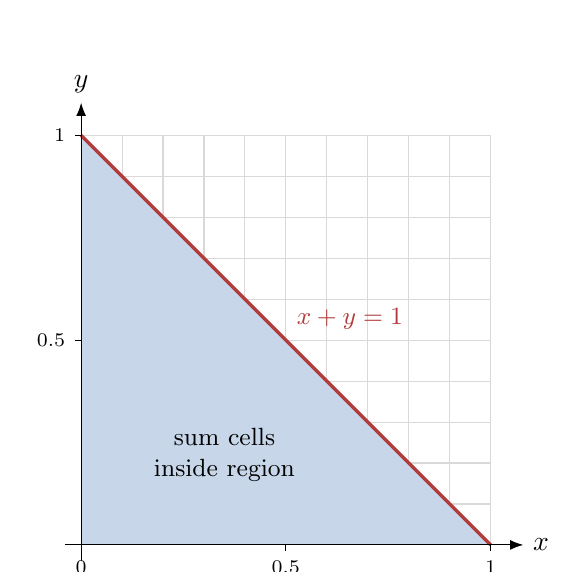
\begin{tikzpicture}[scale=5.2]
  \draw[step=0.1,gray!30,thin] (0,0) grid (1,1);
  \fill[chapterblue!25] (0,0) -- (1,0) -- (0,1) -- cycle;
  \draw[very thick,chapterred] (0,1) -- (1,0) node[midway,above right,font=\small] {$x+y=1$};
  \draw[-Latex] (-0.04,0) -- (1.08,0) node[right] {$x$};
  \draw[-Latex] (0,-0.04) -- (0,1.08) node[above] {$y$};
  \foreach \x in {0,0.5,1} \draw (\x,0) -- +(0,-0.015) node[below,font=\scriptsize] {\x};
  \foreach \y in {0.5,1} \draw (0,\y) -- +(-0.015,0) node[left,font=\scriptsize] {\y};
  \node[font=\small,align=center] at (0.35,0.22) {sum cells\\inside region};
\end{tikzpicture}
\caption{Numerical integration estimates the probability of a region by summing density values over grid cells. The exact answer in Example 24.1 is $1/2$.}
\end{figure}

\section{Change of variables for random variables}

Change of variables is one of the most important applications of the Jacobian. Suppose $(U,V)$ has density $f_{U,V}(u,v)$, and suppose
\[
(x,y)=T(u,v).
\]
If $T$ is one-to-one on the relevant region and has nonzero Jacobian determinant, then the density of $(X,Y)=T(U,V)$ is
\[
f_{X,Y}(x,y)=f_{U,V}(u(x,y),v(x,y))\left|\det\frac{\partial(u,v)}{\partial(x,y)}\right|.
\]
Equivalently, if we integrate in $(u,v)$-coordinates, then
\[
dx\,dy=\left|\det\frac{\partial(x,y)}{\partial(u,v)}\right|du\,dv.
\]
The Jacobian measures local area distortion.

\begin{examplebox}{Example 24.5: Uniform distribution on a disk}
A common mistake is to sample a radius uniformly when trying to sample uniformly from a disk. If $R$ is uniform on $[0,1]$ and $\Theta$ is uniform on $[0,2\pi]$, then points concentrate near the center.

For uniform sampling in the unit disk, use
\[
R=\sqrt U,\qquad \Theta=2\pi V,
\]
where $U,V$ are independent uniform random variables on $[0,1]$. Then
\[
X=R\cos\Theta,\qquad Y=R\sin\Theta.
\]
Why the square root? Because the area of a disk of radius $r$ is proportional to $r^2$, so
\[
\Prob(R\le r)=r^2.
\]
Thus $R^2$ should be uniform on $[0,1]$.
\end{examplebox}

\begin{figure}[H]
\centering
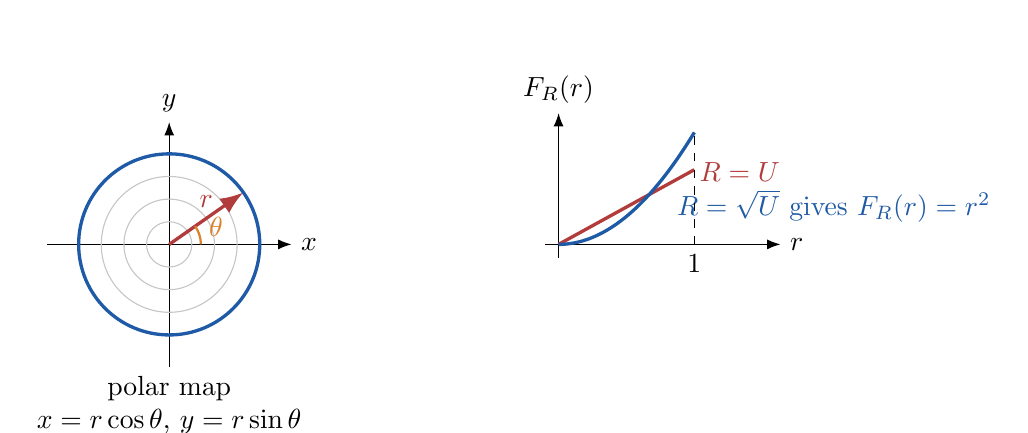
\begin{tikzpicture}[scale=1.15]
  \begin{scope}
    \draw[-Latex] (-1.35,0) -- (1.35,0) node[right] {$x$};
    \draw[-Latex] (0,-1.35) -- (0,1.35) node[above] {$y$};
    \draw[very thick,chapterblue] (0,0) circle (1);
    \foreach \r in {0.25,0.5,0.75} \draw[gray!45] (0,0) circle (\r);
    \draw[vectorred] (0,0) -- (35:1) node[midway,above] {$r$};
    \draw[chapterorange,thick] (0.35,0) arc (0:35:0.35);
    \node[chapterorange] at (20:0.55) {$\theta$};
    \node[below=1.55cm,align=center] {polar map\\$x=r\cos\theta$, $y=r\sin\theta$};
  \end{scope}
  \begin{scope}[xshift=4.3cm]
    \draw[-Latex] (-0.15,0) -- (2.45,0) node[right] {$r$};
    \draw[-Latex] (0,-0.15) -- (0,1.45) node[above] {$F_R(r)$};
    \draw[very thick,chapterred,domain=0:1.5,samples=80] plot (\x,{0.55*\x});
    \node[chapterred,right] at (1.45,0.8) {$R=U$};
    \draw[very thick,chapterblue,domain=0:1.5,samples=80] plot (\x,{0.55*\x*\x});
    \node[chapterblue,right] at (1.2,0.42) {$R=\sqrt U$ gives $F_R(r)=r^2$};
    \draw[dashed] (1.5,0) -- (1.5,1.25);
    \node[below] at (1.5,0) {$1$};
  \end{scope}
\end{tikzpicture}
\caption{Uniform area in a disk requires the radial distribution $\Prob(R\le r)=r^2$, hence $R=\sqrt U$.}
\end{figure}

\section{The bivariate normal distribution}

The multivariate normal distribution is the most important continuous distribution in multivariable statistics. A random vector $X\in\R^n$ has multivariate normal density with mean vector $\mu$ and covariance matrix $\Sigma$ if
\[
f(x)=\frac{1}{(2\pi)^{n/2}|\Sigma|^{1/2}}\exp\left(-\frac12(x-\mu)^T\Sigma^{-1}(x-\mu)\right).
\]
For $n=2$, the level curves of the density are ellipses:
\[
(x-\mu)^T\Sigma^{-1}(x-\mu)=c.
\]
This is a quadratic form. The eigenvectors of $\Sigma$ determine the principal directions of the ellipses, and the eigenvalues determine their squared spread in those directions.

\begin{notebox}[Geometry of covariance]
The covariance matrix is not just a table of numbers. It is a geometric object. It determines the directions and scales of uncertainty.
\end{notebox}

\begin{figure}[H]
\centering
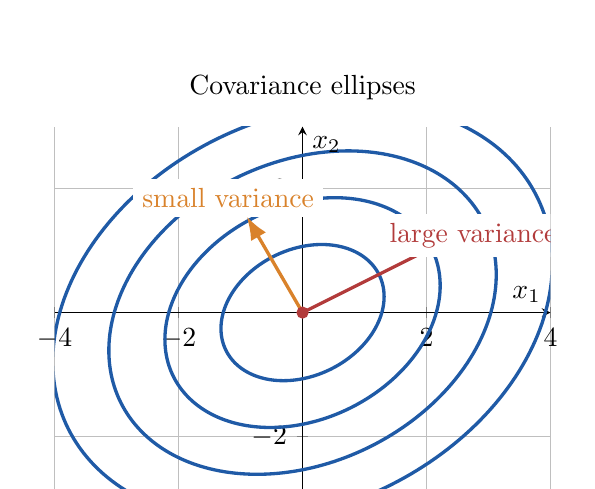
\begin{tikzpicture}
\begin{axis}[
  width=0.68\textwidth,height=0.52\textwidth,
  xmin=-4,xmax=4,ymin=-3,ymax=3,
  axis equal image,
  axis lines=middle,
  xlabel={$x_1$},ylabel={$x_2$},
  grid=both,
  title={Covariance ellipses}
]
\foreach \s in {0.8,1.35,1.9,2.45}{
  \addplot[very thick,chapterblue,domain=0:360,samples=220] ({1.55*\s*cos(x)-0.55*\s*sin(x)},{0.75*\s*cos(x)+1.15*\s*sin(x)});
}
\addplot[only marks,mark=*,mark size=2pt,chapterred] coordinates {(0,0)};
\addplot[chapterred,very thick,-Latex] coordinates {(0,0) (2.4,1.2)};
\addplot[chapterorange,very thick,-Latex] coordinates {(0,0) (-0.9,1.55)};
\node[chapterred,fill=white] at (axis cs:2.75,1.25) {large variance};
\node[chapterorange,fill=white] at (axis cs:-1.2,1.85) {small variance};
\end{axis}
\end{tikzpicture}
\caption{Level curves of a bivariate normal density are ellipses. The covariance matrix controls the directions and scales.}
\end{figure}

\section{Likelihood functions as multivariable functions}

In statistics, the unknown parameter is often a vector
\[
\theta=(\theta_1,\ldots,\theta_p).
\]
Given data $x_1,\ldots,x_n$, the likelihood function is
\[
L(\theta)=f(x_1,\ldots,x_n\mid\theta).
\]
The log-likelihood is
\[
\ell(\theta)=\log L(\theta).
\]
Maximum likelihood estimation asks us to find
\[
\hat\theta=\operatorname*{argmax}_{\theta}\ell(\theta).
\]
This is a multivariable optimization problem.

\begin{examplebox}{Example 24.6: Normal model with unknown mean and variance}
Suppose $x_1,\ldots,x_n$ are modeled as independent normal observations with mean $\mu$ and standard deviation $\sigma>0$. The log-likelihood is, up to an additive constant,
\[
\ell(\mu,\sigma)=-n\log\sigma-\frac{1}{2\sigma^2}\sum_{i=1}^n(x_i-\mu)^2.
\]
The maximum occurs at
\[
\hat\mu=\frac1n\sum_{i=1}^n x_i,
\qquad
\hat\sigma^2=\frac1n\sum_{i=1}^n(x_i-\hat\mu)^2.
\]
This is a two-variable optimization problem on the half-plane $\sigma>0$.
\end{examplebox}

\begin{figure}[H]
\centering
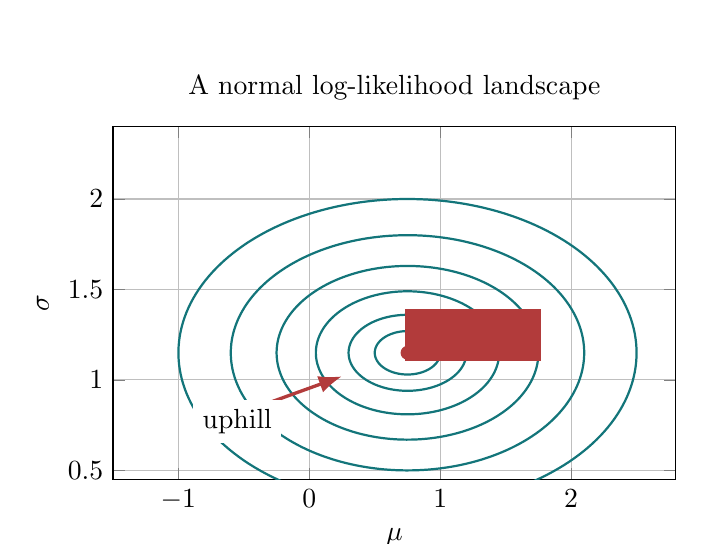
\begin{tikzpicture}
\begin{axis}[
  width=0.72\textwidth,height=0.5\textwidth,
  xmin=-1.5,xmax=2.8,ymin=0.45,ymax=2.4,
  xlabel={$\mu$},ylabel={$\sigma$},
  grid=both,
  title={A normal log-likelihood landscape}
]
\foreach \a/\b in {0.25/0.12,0.45/0.21,0.70/0.34,1.0/0.48,1.35/0.65,1.75/0.85}{
  \addplot[domain=0:360,samples=200,chapterteal!85!black,thick] ({0.75+\a*cos(x)},{1.15+\b*sin(x)});
}
\addplot[only marks,mark=*,mark size=2.3pt,chapterred] coordinates {(0.75,1.15)};
\node[fill=white,chapterred] at (axis cs:1.25,1.25) {$\hat\theta=(\hat\mu,\hat\sigma)$};
\draw[vectorred] (axis cs:-0.4,0.85) -- (axis cs:0.25,1.02);
\node[fill=white] at (axis cs:-0.55,0.77) {uphill};
\end{axis}
\end{tikzpicture}
\caption{A log-likelihood is a function on parameter space. Its maximum gives the maximum likelihood estimate.}
\end{figure}

\section{Score, Hessian, and information}

The gradient of the log-likelihood is called the \textbf{score}:
\[
S(\theta)=\grad\ell(\theta).
\]
At an interior maximum likelihood estimate, the score is zero:
\[
\grad\ell(\hat\theta)=0.
\]
The Hessian matrix is
\[
H(\theta)=\grad^2\ell(\theta).
\]
At a local maximum, the Hessian is usually negative definite. The negative Hessian
\[
-\grad^2\ell(\hat\theta)
\]
measures local curvature of the log-likelihood near the maximum. In many statistical models, this curvature is connected to information and standard errors.

A second-order Taylor approximation gives
\[
\ell(\theta)\approx \ell(\hat\theta)+\frac12(\theta-\hat\theta)^T\grad^2\ell(\hat\theta)(\theta-\hat\theta).
\]
Since the Hessian is negative definite near a maximum, the log-likelihood looks locally like an upside-down quadratic bowl.

\begin{warningbox}[Curvature and uncertainty]
A sharply curved log-likelihood means the parameter is estimated precisely. A flat log-likelihood means the data do not strongly identify the parameter.
\end{warningbox}

\begin{figure}[H]
\centering
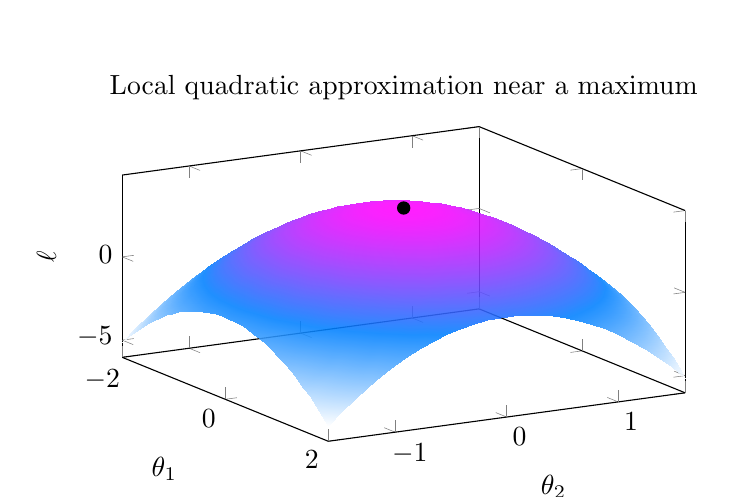
\begin{tikzpicture}
\begin{axis}[
  width=0.72\textwidth,height=0.46\textwidth,
  view={60}{28},
  xlabel={$\theta_1$},ylabel={$\theta_2$},zlabel={$\ell$},
  domain=-2:2,y domain=-1.6:1.6,
  samples=34,samples y=28,
  z buffer=sort,
  colormap/cool,
  title={Local quadratic approximation near a maximum}
]
\addplot3[surf,shader=interp,opacity=0.88] {-x^2-2*y^2+4};
\addplot3[only marks,mark=*,mark size=2.2pt] coordinates {(0,0,4)};
\end{axis}
\end{tikzpicture}
\caption{Near an interior maximum, the second-order Taylor approximation makes the log-likelihood look like an upside-down quadratic bowl.}
\end{figure}

\section{The delta method as linear approximation}

Suppose an estimator $\hat\theta$ is approximately normal:
\[
\hat\theta\approx N(\theta,\Sigma).
\]
If we want to understand $g(\hat\theta)$ for a differentiable function $g$, we use linear approximation:
\[
g(\hat\theta)\approx g(\theta)+\grad g(\theta)^T(\hat\theta-\theta).
\]
Therefore,
\[
\Var(g(\hat\theta))\approx \grad g(\theta)^T\Sigma\grad g(\theta).
\]
This is the multivariable delta method. It is just the linearization from Chapter 9, applied to statistical uncertainty.

\begin{examplebox}{Example 24.7: Ratio of two estimates}
Suppose $\hat\theta=(\hat a,\hat b)$ has covariance matrix $\Sigma$, and we want the uncertainty of
\[
g(a,b)=\frac{a}{b}.
\]
The gradient is
\[
\grad g(a,b)=\left(\frac1b,-\frac{a}{b^2}\right).
\]
So
\[
\Var\left(\frac{\hat a}{\hat b}\right)\approx
\begin{bmatrix}1/b & -a/b^2\end{bmatrix}
\Sigma
\begin{bmatrix}1/b\\ -a/b^2\end{bmatrix}.
\]
\end{examplebox}

\begin{figure}[H]
\centering
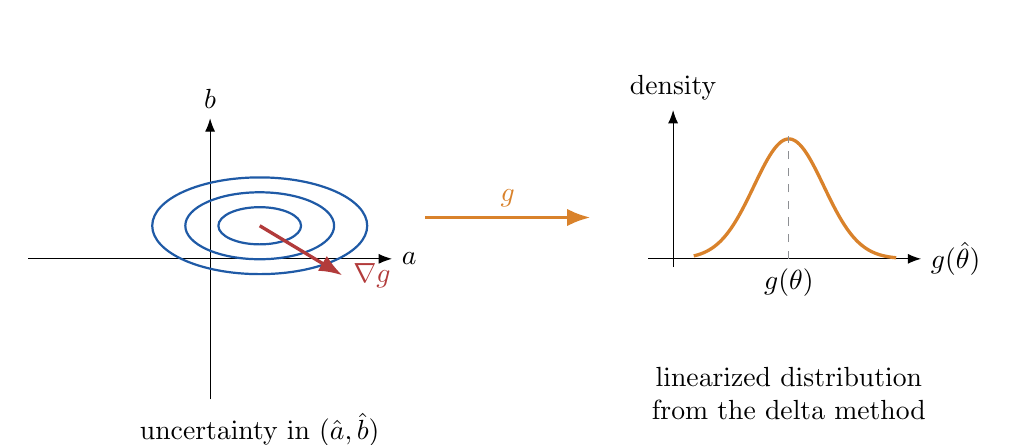
\begin{tikzpicture}[scale=1.05]
  \begin{scope}
    \draw[-Latex] (-2.2,0)--(2.2,0) node[right] {$a$};
    \draw[-Latex] (0,-1.7)--(0,1.7) node[above] {$b$};
    \foreach \s in {0.5,0.9,1.3} \draw[chapterblue,thick] (0.6,0.4) ellipse ({1.0*\s} and {0.45*\s});
    \draw[vectorred] (0.6,0.4)--(1.6,-0.2) node[right] {$\grad g$};
    \node[below] at (0.6,-1.75) {uncertainty in $(\hat a,\hat b)$};
  \end{scope}
  \begin{scope}[xshift=5.6cm]
    \draw[-Latex] (-0.3,0)--(3,0) node[right] {$g(\hat\theta)$};
    \draw[-Latex] (0,-0.1)--(0,1.8) node[above] {density};
    \draw[very thick,chapterorange,domain=0.25:2.7,samples=160] plot (\x,{1.45*exp(-2.8*(\x-1.4)^2)});
    \draw[guide] (1.4,0)--(1.4,1.48);
    \node[below] at (1.4,0) {$g(\theta)$};
    \node[below=1.25cm,align=center] at (1.4,0) {linearized distribution\\from the delta method};
  \end{scope}
  \draw[vectororange] (2.6,0.5) -- (4.6,0.5) node[midway,above] {$g$};
\end{tikzpicture}
\caption{The delta method approximates the distribution of a nonlinear transformation by linearizing the transformation near the mean.}
\end{figure}

\section{Monte Carlo integration}

Monte Carlo integration uses random samples to estimate integrals. If $U_1,\ldots,U_N$ are uniformly sampled from a region $R$ with area $A(R)$, then
\[
\iint_R f(x,y)\dd A\approx A(R)\frac1N\sum_{i=1}^N f(U_i).
\]
If $X_1,\ldots,X_N$ are sampled from a density $p(x)$, then
\[
\E[g(X)]\approx \frac1N\sum_{i=1}^N g(X_i).
\]
This is one of the key computational ideas behind simulation-based statistics, Bayesian computation, and machine learning.

\begin{examplebox}{Example 24.8: Estimating an integral by simulation}
Estimate
\[
I=\int_0^1\int_0^1 e^{-(x^2+y^2)}\dd y\dd x.
\]
If $(U,V)$ is uniform on the unit square, then
\[
I=\E[e^{-(U^2+V^2)}].
\]
So we can approximate $I$ by a sample average.
\end{examplebox}

\begin{figure}[H]
\centering
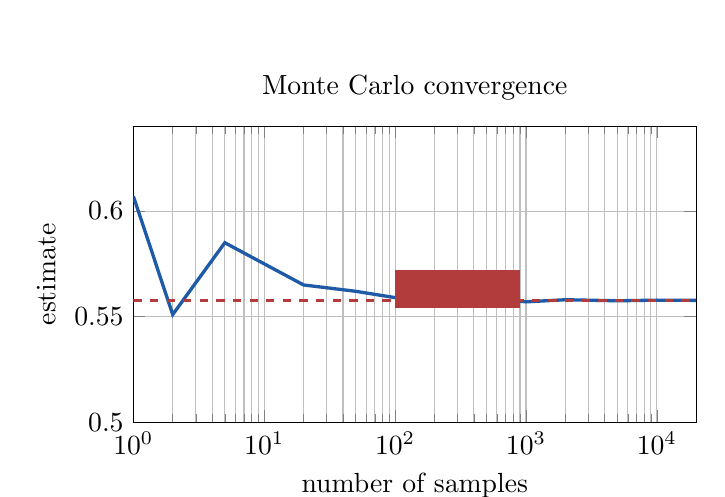
\begin{tikzpicture}
\begin{semilogxaxis}[
  width=0.72\textwidth,height=0.44\textwidth,
  xmin=1,xmax=20000,
  ymin=0.50,ymax=0.64,
  xlabel={number of samples},ylabel={estimate},
  grid=both,
  title={Monte Carlo convergence}
]
\addplot[very thick,chapterblue] coordinates {
(1,0.607) (2,0.551) (5,0.585) (10,0.575) (20,0.565) (50,0.562) (100,0.559) (200,0.561) (500,0.559) (1000,0.557) (2000,0.558) (5000,0.5575) (10000,0.5578) (20000,0.5577)};
\addplot[chapterred,dashed,very thick] coordinates {(1,0.5577) (20000,0.5577)};
\node[fill=white,chapterred] at (axis cs:300,0.563) {reference};
\end{semilogxaxis}
\end{tikzpicture}
\caption{Monte Carlo integration estimates an integral by averaging random function values. The estimate stabilizes as the sample size grows.}
\end{figure}

\section{Bayesian posterior as a normalized density}

Bayesian statistics combines a likelihood and a prior distribution. If $\theta$ is a parameter and $x$ is observed data, Bayes' rule gives
\[
p(\theta\mid x)=\frac{p(x\mid\theta)p(\theta)}{p(x)}.
\]
The denominator
\[
p(x)=\int p(x\mid\theta)p(\theta)\dd\theta
\]
is a normalizing constant. In multivariable problems,
\[
p(x)=\int_{\Theta}p(x\mid\theta)p(\theta)\dd\theta
\]
may be a high-dimensional integral. This is why numerical integration, Monte Carlo methods, and optimization are so important in modern Bayesian statistics.

\begin{examplebox}{Example 24.9: A two-parameter posterior landscape}
Suppose a posterior density for two parameters is proportional to
\[
\exp\left[-\frac12(\theta-\mu)^TA(\theta-\mu)\right].
\]
The contours are ellipses. The matrix $A$ is a precision matrix, and $A^{-1}$ is the covariance matrix.
\end{examplebox}

\begin{figure}[H]
\centering
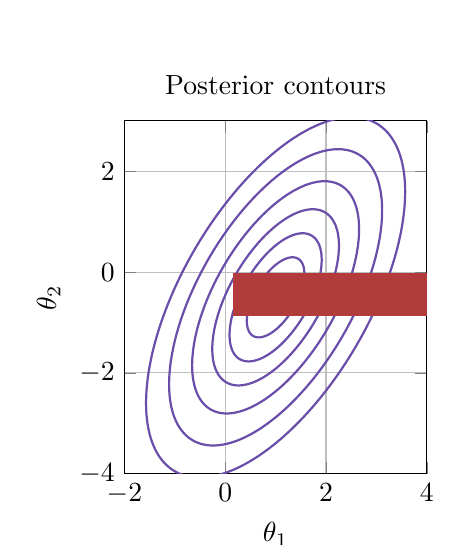
\begin{tikzpicture}
\begin{axis}[
  width=0.70\textwidth,height=0.50\textwidth,
  xmin=-2,xmax=4,ymin=-4,ymax=3,
  axis equal image,
  xlabel={$\theta_1$},ylabel={$\theta_2$},
  grid=both,
  title={Posterior contours}
]
\foreach \s in {0.5,0.8,1.1,1.45,1.85,2.25}{
  \addplot[domain=0:360,samples=220,chapterpurple,thick] ({1+1.05*\s*cos(x)+0.45*\s*sin(x)},{-0.5+0.35*\s*cos(x)+1.55*\s*sin(x)});
}
\addplot[only marks,mark=x,mark size=4pt,very thick,chapterred] coordinates {(1,-0.5)};
\node[fill=white,chapterred] at (axis cs:2.15,-0.45) {posterior mode};
\end{axis}
\end{tikzpicture}
\caption{A two-parameter posterior density. The highest point is the posterior mode, and the contour shape describes uncertainty.}
\end{figure}

\section{What to remember}

Multivariable calculus gives statistics its geometry and computation.
\begin{itemize}
  \item A joint density is a nonnegative function with total integral $1$.
  \item A probability is an integral over a region.
  \item A marginal density is obtained by integrating out variables.
  \item A conditional density is a normalized slice of the joint density.
  \item An expectation is an integral of a function against a density.
  \item A covariance matrix is a geometric object describing spread and direction.
  \item A Jacobian accounts for local volume distortion under a change of variables.
  \item A likelihood is a function on parameter space.
  \item A score is the gradient of a log-likelihood.
  \item A Hessian describes local curvature and uncertainty.
  \item Monte Carlo methods approximate integrals by random averages.
\end{itemize}

\section{Python lab}

In the accompanying lab, you will:
\begin{enumerate}
  \item plot joint densities as surfaces and contour maps;
  \item compute marginal and conditional densities numerically;
  \item simulate points from a disk using the correct radial transformation;
  \item visualize covariance ellipses of a bivariate normal distribution;
  \item plot a normal log-likelihood surface for unknown mean and variance;
  \item approximate a nonlinear estimator using the delta method;
  \item estimate probabilities and expectations using Monte Carlo simulation.
\end{enumerate}

\begin{notebox}[Chapter resources]
\begin{itemize}
  \item Lab notebook: \url{../labs/chapter-24-multivariable-calculus-for-probability-and-statistics.ipynb}
  \item Interactive page: \url{../htmls/chapter-24-multivariable-calculus-for-probability-and-statistics.html}
\end{itemize}
\end{notebox}

\section{Exercises}

\subsection*{Conceptual questions}
\begin{enumerate}
  \item Explain why a joint density must integrate to $1$.
  \item In your own words, explain the difference between a marginal density and a conditional density.
  \item Why is a covariance matrix a geometric object?
  \item Why does a change of variables formula need a Jacobian factor?
  \item What is the difference between likelihood and probability?
  \item Explain why the gradient of the log-likelihood is zero at an interior maximum likelihood estimate.
  \item Explain how the Hessian of the log-likelihood is related to uncertainty.
  \item What does Monte Carlo integration estimate, and why does it work?
\end{enumerate}

\subsection*{Computation and derivation}
\begin{enumerate}
  \item Let $f(x,y)=2$ on the triangle $0\le y\le x\le 1$ and $0$ elsewhere. Verify that $f$ is a joint density.
  \item For the density in Problem 1, compute $f_X(x)$ and $f_Y(y)$.
  \item For the density in Problem 1, compute $\Prob(Y\le 1/2)$.
  \item Let $f(x,y)=4xy$ on $0\le x\le 1$, $0\le y\le 1$. Find the marginal densities. Are $X$ and $Y$ independent?
  \item Let $f(x,y)=c(x^2+y^2)$ on the unit disk. Find $c$.
  \item For independent uniform random variables $U,V$ on $[0,1]$, define $X=U+V$. Find the density of $X$ by geometric reasoning.
  \item Let $X,Y$ have joint density $f(x,y)=x+y$ on the unit square. Compute $\E[X^2]$.
  \item Let $X,Y$ have joint density $f(x,y)=x+y$ on the unit square. Compute $\Var(X)$.
  \item Let $X,Y$ be independent standard normal random variables. Use polar coordinates to evaluate
  \[
  \int_{-\infty}^{\infty}\int_{-\infty}^{\infty}e^{-(x^2+y^2)/2}\dd x\dd y.
  \]
  \item Suppose $X$ has density $f_X(x)=2x$ on $0\le x\le 1$, and $Y=X^2$. Find the density of $Y$.
\end{enumerate}

\subsection*{Likelihood and approximation}
\begin{enumerate}
  \item For Bernoulli data with $k$ successes in $n$ trials, the log-likelihood is
  \[
  \ell(p)=k\log p+(n-k)\log(1-p).
  \]
  Find the maximum likelihood estimate of $p$.
  \item Compute the second derivative of the Bernoulli log-likelihood and evaluate it at $\hat p=k/n$.
  \item For normal data with known variance $\sigma^2$, derive the maximum likelihood estimate of $\mu$.
  \item For normal data with unknown mean and variance, explain why the log-likelihood is a function of two variables.
  \item Let $g(a,b)=a/b$. Compute the linear approximation of $g$ at $(2,1)$.
  \item Let $\Sigma=\begin{bmatrix}4&1\\1&2\end{bmatrix}$. For $g(a,b)=a/b$, approximate the variance of $g(\hat a,\hat b)$ at $(a,b)=(2,1)$ using the delta method.
  \item Let $\ell(\theta_1,\theta_2)=-(\theta_1-1)^2-4(\theta_2+2)^2$. Find the maximum and the Hessian.
  \item Explain how the contours of the function in Problem 7 describe uncertainty.
\end{enumerate}

\subsection*{Python exercises}
\begin{enumerate}
  \item Numerically verify that $f(x,y)=x+y$ integrates to $1$ on the unit square.
  \item Use Monte Carlo simulation to estimate $\Prob(X+Y\le 1)$ for the density $f(x,y)=x+y$ on the unit square. Compare with the exact answer.
  \item Write code to plot the bivariate normal density for several covariance matrices.
  \item Simulate uniform points in the unit disk using both $R=U$ and $R=\sqrt U$. Compare the radial histograms.
  \item Generate normal data and plot the log-likelihood contours for $(\mu,\sigma)$.
  \item Simulate the delta method example for different covariance matrices.
  \item Estimate $\int_0^1\int_0^1\sin(xy)\dd y\dd x$ by Monte Carlo simulation.
  \item Use finite differences to approximate the gradient and Hessian of a two-parameter log-likelihood.
\end{enumerate}

\section{Chapter summary}

This chapter showed how the main ideas of multivariable calculus become tools for probability and statistics. Densities are functions integrated over regions. Expectations are weighted integrals. Marginalization is integration over unused variables. Change of variables requires Jacobians. Likelihood functions are multivariable functions on parameter space, and their maxima are studied using gradients and Hessians. Taylor approximation explains why many estimators are approximately normal and why curvature measures uncertainty. These ideas prepare us for statistical theory, Bayesian inference, data science, and machine learning.

\end{document}
